In this section we present a novel program to test the Higgs couplings \emph{off-shell} and at high-energy, via their contributions to the physics of longitudinally polarized gauge bosons. We will show that this program is potentially competitive with \emph{on-shell} measurements, but it also offers endless opportunities of refinements and improvements. 


Our leitmotiv is that \emph{any} observable modification of a SM coupling will produce in \emph{some} process a growth with energy. In some sense, this is obvious: since the SM is the only theory that can be extrapolated to arbitrarily high-energy, any departure from it can have only a finite range of validity, a fact that is made manifest by a disproportionate growth in some scattering amplitude. Theories with a finite range of validity are, by definition, EFTs; for this reason the best vehicle to communicate our message is  the EFT language where deviations on Higgs couplings come from the operators $\op_{BB},\op_{WW},\op_{y_t},\op_{6}$, etc. We stress nevertheless that at, tree level, the very same conclusions can be reached in the $\kappa$ framework \cite{Heinemeyer:2013tqa} or in the unitary-gauge framework of Ref.~\cite{deFlorian:2016spz,Gupta:2014rxa}.



The operators of that we will be interested on have the form $|H|^2\times \op^{\mathrm SM}$, with $\op^{\mathrm SM}$ a dimension-4  SM operator (i.e. kinetic terms, Higgs potential, and Yukawas) times
\begin{equation}
|H|^2=\frac{1}{2}\left(v^2+ 2 hv + h^2+2\phi^+\phi^-+(\phi^0)^2\right)
\end{equation}
where $h$ is the physical Higgs boson and $\phi^{\pm,0}$ are the would-be longitudinal polarizations of $W$- and $Z$- bosons.
In this contribution we focus on the last two terms, and study processes with longitudinal gauge bosons instead of processes with an on-shell Higgs; we dub this search strategy ``Higgs without Higgs''  - HwH in short \cite{Henning:2018kys}.  
%
For each modification of a Higgs coupling we identify a process where couplings different from the SM ones induce a high-energy growth in the amplitude with respect the SM,
\begin{eqnarray}
&&\kappa_t: p p \to j t+ V_LV^\prime_L\label{prockt}\\
&&\kappa_\lambda:  p p \to  j j h + V_LV^\prime_L\,,\hspace{.3cm}p p \to jj+4V_L, \label{prockh36}\\
 &&\kappa_{\gamma\gamma,Z\gamma}:  p p \to j j +V^\prime V,\label{prockga} \\ 
&&\kappa_V:  p p \to jj+V_LV^\prime_L,\label{prockv}\\
&&\kappa_g:  p p \to W_L^+W_L^-, Z_LZ_L ,\ \label{prockg}
\end{eqnarray} 
where $V_LV^\prime_L\equiv\{W_L^\pm W_L^\pm,W_L^\pm W_L^\mp,W_L^\pm Z_L,Z_LZ_L\}$ (similarly $4V_L$ a generic longitudinaly polarized final state) and $V^{(\prime)}$ any (longitudinal or transverse) vector, including photons.
In the following paragraphs we explore these processes in turn and provide a first estimate of the potential HwH reach at the HL-LHC in comparison with the reach from Higgs couplings measurements. 
Our results are based on leading order (LO) MadGraph simulations \cite{Alwall:2014hca}, where the Higgs couplings have been modified using FeynRules \cite{Christensen:2008py} and checked against the model of Ref. \cite{Falkowski:2015wza}.
%Before concluding we comment on the extension of this program to future colliders.

 


 %\begin{widetext}
\begin{figure}[t]
\begin{center}
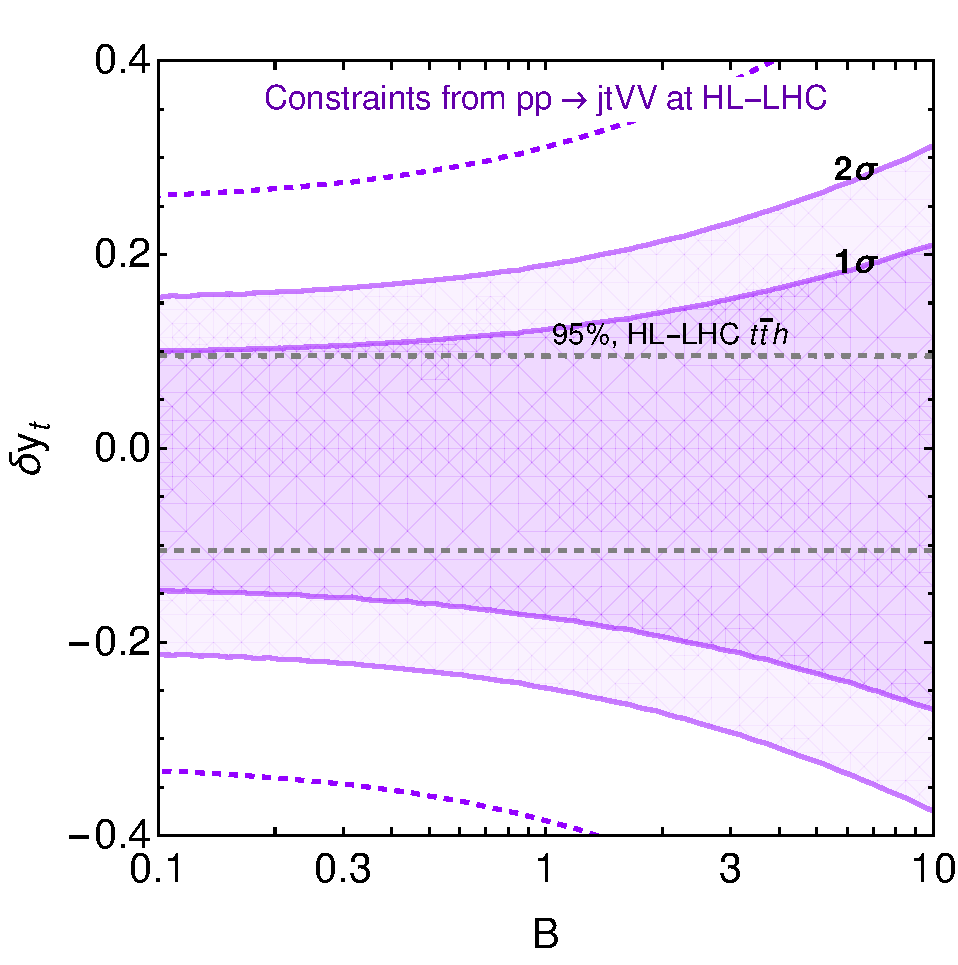
\includegraphics[width=0.32\textwidth]{\main/section4/plots/ytHwHconstraint.pdf}
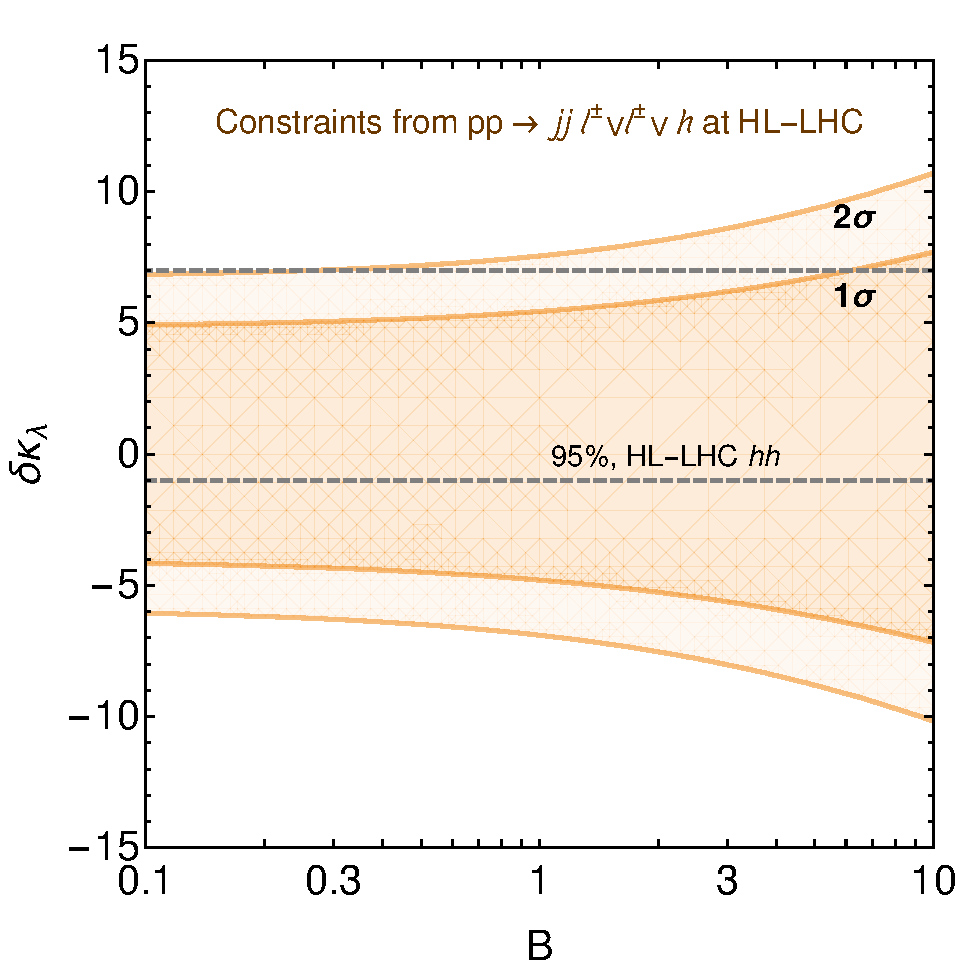
\includegraphics[width=0.32\textwidth]{\main/section4/plots/hhhfromjjwwh.pdf}
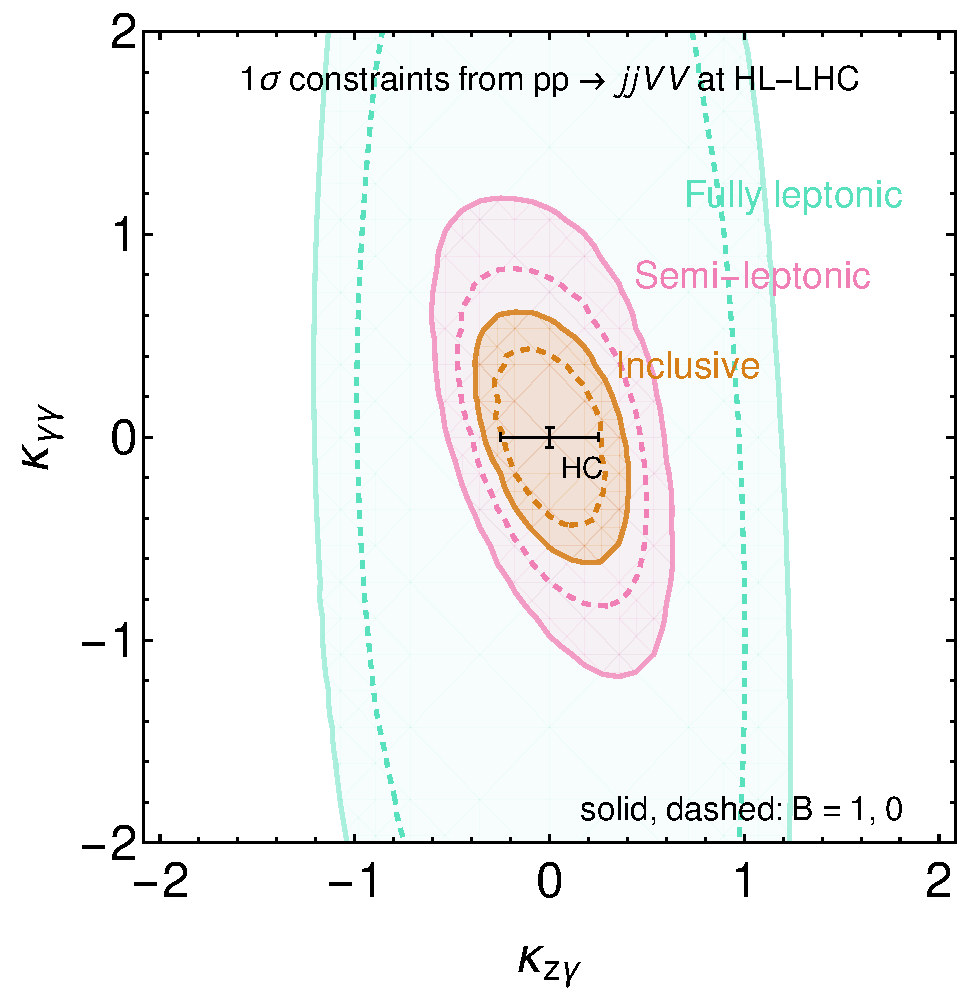
\includegraphics[width=0.30\textwidth]{\main/section4/plots/hhvv_constraints.pdf}
\end{center}
     \caption{\footnotesize \emph{LEFT: HL-LHC (3000 fb$^{-1}$) sensitivity on modifications of the top quark Yukawa $\delta y_t$ from the process in \eq{prockt} (shaded bands), and from measurements of Higgs couplings (95\%C.L., dashed grey lines); $B$ controls additional backgrounds (for $B=1$ the analysis includes a number of background events equal to the SM signal); $1\sigma$ results without the $0\ell$ and $1\ell$ categories correspond to the dashed purple line. CENTER: same but for modifications of the Higgs trilinear $\delta\kappa_\lambda$. RIGHT: $1\sigma$ reach for modification of the Higgs-$\gamma\gamma$ and $Z\gamma$ rates, using high-$E$ measurements (green,pink,brown bands correspond to leptonic,semileptonic, and also hadronic final states)  or Higgs couplings (black error bars). 
}}\label{fig:reach}
\end{figure} 
%\end{widetext}




\vspace{5mm}
\noindent
{\bf The top Yukawa.}
Modifications of the Yukawa coupling of the Higgs boson to top quarks is reputedly difficult to measure on the $h$ resonance~\cite{Aaboud:2018urx}; however, an anomalous top quark Yukawa induces a quadratic energy growth in the five point amplitude involving a bottom quark, a top, and three longitudinal bosons $W_LV_LV_L$. This amplitude leads to a process with a final state consisting of a top quark, a forward jet and two longitudinally polarized vector bosons in the final state.\footnote{See also Ref.~\cite{Degrande:2018fog} that  studies $thj$ final states which exhibits linear $E$-growth with modifications of the top-Yukawa.}

 The top carries a large transverse momentum $p_T^t$ due to the hardness of the process, which makes it a good discriminator. We consider two categories, for $p_T^t>250(500)$~GeV. A forward jet with $|\eta_j|>2.5$, $p_T^j>30$~GeV and $E_j>300$ GeV is required. The signal is classified by  counting the number of extra leptons reconstructed in the event. The following table shows the number of signal events  at the 14 TeV HL-LHC  with 3000 fb$^{-1}$, for $p_T^t>250$~GeV / $p_T^t>500$~GeV,
  

\begin{center}
\begin{tabular}{|c|c|c|c|c|c|}
\hline
Process& 0$\ell$ & 1$\ell$ & $\ell^\pm\ell^\mp$ & $\ell^\pm\ell^\pm$ & $3\ell(4\ell)$\\
 \hline
 $W^\pm W^\mp$    &  3449/567 & 1724/283 & 216/35 & - & -  \\
 $W^\pm W^\pm$    &  2850/398 & 1425/199 & - & 178/25 & -  \\
 $W^\pm Z$   &  3860/632& 965/158 & 273/45 & - & 68/11 \\
 $Z Z$    &  2484/364& - & 351/49 & - &  (12/2) \\\hline
\end{tabular}
 \end{center}
 
The categories with two or more leptons have small background.
%
The largest source of background for the hadronic modes comes from $\bar t t jj\to tWbjj$ where a $bj$ pair is taken to reconstruct a $W/Z$-boson.
The initial $\bar{t}tjj$ cross section is approximately six orders of magnitude bigger than the ones we are interested in, but we have verified that simple cuts on the invariant mass of the $bj$ pair, on the rapidity of the forward jet, on $p_T^t$, and on the separation between the $W$ and the $b$, as well as vector boson tagging techniques \cite{ATLAS-CONF-2018-016}, can reduce this background to a level that is comparable with the signal.

We broadly parametrize this and other backgrounds by a uniform rescaling $B$ of the SM signal expectation in each bin (so that for $B=1$ we add an irreducible background equal to the SM signal in each channel), and show the estimated reach in the left panel of Fig.~\ref{fig:reach}. The dashed grey lines compare our results with those from HC measurements~\cite{HLHEReport}. For illustration we also show  results that focus on channels with at least 2 leptons with a dashed purple line: here the backgrounds are much smaller. The large number of events left in the zero and one lepton categories makes it possible to extend the analysis to higher energies, where not only the effects of the energy growth will be enhanced, but also the background reduced.






\vspace{5mm}
\noindent
{\bf The Higgs self coupling.}
Measurements of the Higgs self-coupling have received enormous attention in collider studies.  In the di-Higgs channel at HL-LHC precision can reach $\delta\kappa_\lambda\in[-1.8,6.7]$ at 95\%C.L.~\cite{ATL-PHYS-PUB-2017-001} using the $b\bar{b}\gamma\gamma$ final state. 
Here we propose the processes of Eq.~(\ref{prockh36}) with VBS scattering topology and a  multitude of longitudinally polarized vector bosons.
The modified coupling $\delta \kappa_\lambda$, or the operator $\op_6$, induces a linear growth  with energy w.r.t. the SM in processes with $jj h V_LV_L $ final state, and a quadratic growth in processes with  $jj V_LV_LV_LV_L$. For the former, the same-sign $W^\pm W^\pm h jj$  with leptonic $(e,\mu)$ decays is particularly favourable for its low background: two same-sign leptons (2ssl) and VBS topology offers a good discriminator against background, allowing for $h\to\bar b b$ decays. For illustration we focus on this channel in which the SM gives $N_{\textrm{SM}}\simeq 50$ events. {Backgrounds from $ t \bar t jj$ enter with a mis-identified lepton, but it can be shown that they can be kept under control with the efficiencies reported in \cite{Khachatryan:2015hwa} and with VBS cuts on the forward jets. A potentially larger background is expected to come from fake leptons, but the precise estimation of it is left for future work.}


The results -shown in the center panel of Fig.~\ref{fig:reach}- are very encouraging: this simple analysis can match the precision of the by-now very elaborate di-Higgs studies.
There are many directions in which this approach can be further refined: \emph{i)} including the  many other final states, both for the vector decays and for the Higgs decay \emph{ii)} including the  $E^2$-growing $jj V_LV_LV_LV_L$ topologies, \emph{iii)} taking into account differential information.
Moreover, the process studied grows only linearly with energy w.r.t. the SM amplitude with transverse vectors in the final state, but it grows quadratically w.r.t. the SM final states, so \emph{iv)} measurements of the polarization fraction can improve this measurement.



\vspace{5mm}
\noindent
{\bf Higgs to $\gamma\gamma,Z\gamma$.}
These decay rates are loop-level and small in the SM: their measurement implies therefore  tight constraints on possible large (tree-level) BSM effects, which in the EFT language are captured by the operators $\op_{WW,BB}$.\footnote{The same operators also affect the  $h$ couplings to $Z_TZ_T$ and $W_TW_T$. The same qualitative analysis can be performed with focus on the $hA_{\mu\nu}A^{\mu\nu}$ and  $hA_{\mu\nu}Z^{\mu\nu}$ vertices, but we prefer to work here with the gauge invariant $\op_{WW,BB}$ operators.}
These also enter in high-energy VBS \eq{prockga}, and they represent a beautiful additional motivation (together with $\kappa_V$, see below) to study these processes, which at present are often interpreted in the context of anomalous quartic gauge couplings (QGC)~\cite{Eboli:2006wa}, corresponding to dimension-8 operators.

We perform a simple analysis of vector boson scattering (VBS) with $W^\pm W^\pm, ZZ, WZ,Z\gamma$ final states. For the first three we use the usual cuts on the forward jets: $|\delta_{jj}|>2.5$, $p_T^j>30$~GeV and $m_{jj}>500$~GeV \cite{Aad:2014zda}. A kinematic variable that captures the hardness of the $2\to 2$ process is the scalar sum of the $p_T^V$ of the vector bosons, and therefore we bin the distribution in bins of 250 GeV up to 2 TeV. For the $Z\gamma$ final state, we follow the analysis for aQGC of \cite{Aaboud:2017pds}.

The combined results are displayed in the right panel of Fig.~\ref{fig:reach}, for fully leptonic, semileptonic and fully hadronic decays, for backgrounds  $B=0,1$ where, as explained above, $B=1$ corresponds to an additional background of the same order as the SM. Note that we translated the constraints on $c_{BB},c_{WW}$ to the $\kappa_{\gamma\gamma},\kappa_{z\gamma}$. We find that the $ZZ,Z\gamma$ final states provide the best reach.
For comparison, the individual reach from HL-LHC measurements of HC \cite{HLHEReport} is shown by the black error bars. These clearly offer an unbeatable sensitivity in the $h\gamma\gamma$ direction; the $hZ\gamma$ direction is however less tested, and our simple analysis of high-energy probes shows promising results.



\vspace{5mm}
\noindent
{\bf Higgs to $W^+W^-,ZZ$.}
It is  known that modifications of the tree-level $hZZ$ and $hW^+W^-$ SM couplings (assumed here to be controlled by a unique parameter, corresponding for instance to $\op_H$ in the SILH basis \cite{Giudice:2007fh}) imply a quadratic $E$-growth in longitudinal VBS. This is discussed in detail in Ref.~\cite{Contino:2010mh} (and \cite{Contino:2013gna} for linear colliders), where it is pointed out that, in the SM, the longitudinal component is suppressed by an accidental factor $\sim 2000$, which is equivalent to a very large irreducible background. This motivated studies of VBS $hh$ pair production instead, see \cite{Bishara:2016kjn}, finding at $1\sigma$, $\delta\kappa_V\lesssim 8\%$, comparable to $\delta\kappa_V\lesssim 5\%$ from HC \cite{HLHEReport}.\footnote{The authors of \cite{Bishara:2016kjn} assume separate couplings of the vector bosons to $h$ or $h^2$; when the Higgs is part of a doublet, these are proportional. Moreover, the numbers we report here are indicative: both HC measurements and the di-higgs analysis have  optimistic and pessimistic scenarios in which these numbers might differ.}




\vspace{5mm}
\noindent
{\bf Higgs to $gg$.}
This coupling modifies the main production mode at hadron colliders and is, therefore, very well measured. 
The most interesting high-energy process that can be associated with this coupling is $gg\to ZZ$, which has  been discussed in Refs.~\cite{Azatov:2014jga,Cacciapaglia:2014rla,Azatov:2016xik}. 
Using the results from Ref.~\cite{Azatov:2014jga} we estimate HwH versus HC reach at the end of the HL-LHC, in particular we have considered a scenario with and one without the background and three different decay channels . We find that 
\begin{eqnarray}
&\textrm{HC:}\,\,\,\, & |\kappa_g|\lesssim 0.025\nn\\
&\textrm{HwH:}&|\kappa_g| \lesssim 0.24\, /\, 0.06 \, /\, 0.01\\
&\textrm{HwH}&(\textrm{no }\bar qq\to Z_TZ_T):\,\, |\kappa_g| \lesssim 0.09  \, /\, 0.02  \, /\, 0.005\nn
\end{eqnarray}
where the numbers stand for the fully leptonic / semileptonic / fully hadronic channels.

The partonic $\bar qq\to Z_TZ_T$ process represents here the main irreducible background, as it does not interfere with our $gg\to Z_LZ_L$  amplitude with longitudinal polarization. Its reduction would constitute an important aspect of HwH analyses. Notice that, unfortunately, in the SM  the $gg\to Z_LZ_L$ process is extremely suppressed at high-$E$, to the benefit of the transverse $TT$ one, see Ref.~\cite{Glover:1988rg}.  This implies that the $SM-BSM$ interference is also suppressed.

Despite these difficulties, which might be overcome in more refined analyses (along the lines of \cite{Panico:2017frx,Azatov:2017kzw}), the high-$E$ results remain competitive  in the semileptonic and fully hadronic channels, assuming that the background from $\bar qq\to Z_TZ_T$ can be efficiently suppressed. 

\vspace{1cm}

In summary, the preliminary results are very positive,
 especially given the potential of improvements that we foresee.  
Simple cut-and-count analyses were shown, in some cases, to match the precision of sophisticated Higgs Coupling measurements.
For instance, the $jjW^\pm W^\pm h$  channel with leptonic decays, allows a precision comparable to di-Higgs production in measuring the Higgs self-coupling. Similarly, modifications of the top Yukawa can be measured in  the many $j t+ V_LV^\prime_L$ final states to a precision in the ballpark of Higgs coupling measurements.
VBS processes and $ZZ$ at high-energy offer further alternative possibilities to test the Higgs coupling to electroweak gauge bosons and to gluons, respectively.

